%% bare_jrnl.tex
%% V1.3
%% 2007/01/11
%% by Michael Shell
%% see http://www.michaelshell.org/
%% for current contact information.
%%
%% This is a skeleton file demonstrating the use of IEEEtran.cls
%% (requires IEEEtran.cls version 1.7 or later) with an IEEE journal paper.
%%
%% Support sites:
%% http://www.michaelshell.org/tex/ieeetran/
%% http://www.ctan.org/tex-archive/macros/latex/contrib/IEEEtran/
%% and
%% http://www.ieee.org/

%%*************************************************************************
%% Legal Notice:
%% This code is offered as-is without any warranty either expressed or
%% implied; without even the implied warranty of MERCHANTABILITY or
%% FITNESS FOR A PARTICULAR PURPOSE!
%% User assumes all risk.
%% In no event shall IEEE or any contributor to this code be liable for
%% any damages or losses, including, but not limited to, incidental,
%% consequential, or any other damages, resulting from the use or misuse
%% of any information contained here.
%%
%% All comments are the opinions of their respective authors and are not
%% necessarily endorsed by the IEEE.
%%
%% This work is distributed under the LaTeX Project Public License (LPPL)
%% ( http://www.latex-project.org/ ) version 1.3, and may be freely used,
%% distributed and modified. A copy of the LPPL, version 1.3, is included
%% in the base LaTeX documentation of all distributions of LaTeX released
%% 2003/12/01 or later.
%% Retain all contribution notices and credits.
%% ** Modified files should be clearly indicated as such, including  **
%% ** renaming them and changing author support contact information. **
%%
%% File list of work: IEEEtran.cls, IEEEtran_HOWTO.pdf, bare_adv.tex,
%%                    bare_conf.tex, bare_jrnl.tex, bare_jrnl_compsoc.tex
%%*************************************************************************

\documentclass[journal]{IEEEtran}

\newcommand{\subparagraph}{}
\def\naive{na\"{\i}ve}

\usepackage{amsmath,
            amssymb,
            amsthm,
            atbegshi,
            caption,
            epigraph,
            etoolbox,
            enumitem,
            fancyhdr,
            framed,
            graphicx,
            hyperref,
            kpfonts,
            lipsum,
            longtable,
            subcaption,
            tabulary,
            thmtools,
            tikz,
            tikzpagenodes,
            titletoc,
            titlesec,
            tocloft,
            url,
            wrapfig
}
\usepackage[square,sort,comma,numbers]{natbib}
\usepackage[utf8]{inputenc}
\usepackage[left=2.1cm,right=2.1cm,bottom=3cm]{geometry}
\usetikzlibrary{arrows}

\DeclareMathOperator*{\argmax}{\arg\!\max}

\tikzset{%
    treenode/.style = {align=center, inner sep=0pt, text centered,
    font=\sffamily},
    arnN/.style = {treenode, circle, white, font=\sffamily\bfseries,
    draw=black, fill=black, text width=3.5em},
    arnR/.style = {treenode, circle, red, draw=red,
    text width=2.9em, very thick},% arbre rouge noir, noeud rouge
}

\begin{document}
%
% paper title
% can use linebreaks \\ within to get better formatting as desired
\title{2048 Expectimax Solver}

\author{Anders Sildnes, Andrej Leitner~\IEEEmembership{students at NTNU}% <-this % stops a space. jobtitle in memberkj
}% \thanks{Utsendt 2014}}

% The paper headers
\markboth{2048 Expectimax Solver}%
{h}

% make the title area
\maketitle

\begin{abstract}
    This text answers assignment 5: writing a solver for the game 2048.
    We present a solver using Expectimax algorithm. We explain our choice of
    heuristics and results.
\end{abstract}

% \begin{IEEEkeywords}
%     2048, expectimax, IT3105
% \end{IEEEkeywords}
\IEEEPARstart{T}{he} purpose of ``2048'' is to slide tiles with numbers
$2^{n}$, and join them together to form 2048 ($2^{11}$), or possibly higher.
Between each slide, i.e.\ moving all the tiles on the board north, west, east
or south, a random tile valued either 2 or 4 appears on the board, which adds
difficulty in solving the game.
% It can be thought of as a 2-player, turn-based game. 
% The opponent places tiles valued either $2$ or $4$ in an availible location.
% Then, the other player makes a move to slide all tiles in a given direction.
% This goes back and forth until there are no more availible moves.

% In a turn-based game, you have the time to consider the consequences for each possible
% action. This gives computers immense advantages over humans:
% IBM's chess-solving machine ``Deep Blue'' won against Garry Kasparov in 1997 considered more than
% 200 million possible moves per second\footnote{Info taken from lecture slides}.
% In the case of 2048, this could yield a valid solution in a short amount of
% time. However, not everyone has access to such fast hardware and
% multi-threading so a way to prune the search space is needed.

\section*{Assumptions}
It is possible to obtain tiles values up to $2^{14}$ within reasonable time.
Our assignment bounds, however, did not require us to achieve such a high level
of performance:
\begin{enumerate}
    \item The highest value tile does not need to exceed 4096 ($2^{12}$).
    \item Execution time is not critical (acceptable as long as $< 10$ minutes)
\end{enumerate}
This implies that our chosen heuristic and solver method does not need a strong
level of optimization to work. Indeed, the work of~\cite{brutesolver} shows that
a \naive{} search can be used to solve the game within the bounds listed above.
Still, we have implemented an expectimax approach which is much more scalable.

\section*{Minimax Algorithm}
The purpose of minimax is to minimize loss for a worst possible scenario.
This means choosing an action such that your opponent can do ``least amount of damage'',
i.e.\ leaving you in a promising state. The process of to determine the best
action available given your opponent's possible re-action is also referred to as 
\textit{adversarial search}.
For 2048 this would mean always making a move such that no matter where the next
tile goes, and no matter what value, your action minimizes loss.

% PERFECT INFORMATION
% DISCRETE SPACE
% PLY

2048, however, is a stochastic game. The opponent will never intelligently
select a bad location or value. Therefore, we felt that minimax, which always prepares
for the worst case, is too pessimistic in its choice of actions. Furthermore, the
distribution of tiles are given: there is a 90\% chance of getting a
tile valued 2, and 10\% chance of getting a tile valued 4. Thus, it is possible
to make somewhat accurate predictions about the expected likelihood of future states of the
game. What cannot be predicted is the location of new tiles. However, the possible
locations are typically not many enough so that an adversarial search cannot completely
explore the possible outcomes.


Minimax with probabilistic values to each state leads to the modified \textit{expectimax} algorithm.
Search space is expanded similar to in minimax, but it is extended with 
\textit{chance nodes}.  The chance nodes considers each possible successor states, but instead
of considering the value from each board/objective function, it also takes into account 
the probability of getting each state.
Their importance is that if an action might lead to a bad, but unlikely result,
this result will not significantly reduce the overall value of the action.

\section*{Heuristic}

To assess whether or not a current game state is good or not, we have one
heuristic function that assesses how promising a given board is. 
Our heuristic is based on ideas we found online and through some play of our
own.

\subsection*{Gradients}
If a large value is in the middle of the board, it will be hard to pair up
with other adjacent tiles. Therefore, we would like to set a natural preference
for having larger values clustered in a corner. This way, they do not interfere
with other lower-valued tiles. However, having large values
in separate corners implies that there are lower valued tiles between them.
This makes the board hard to maneuver and reduces the possible spaces. 
Therefore, we want to penalize the score when values are spread out.

To calculate the value of a board, we apply a $4\times{}4$ mask and retrieve the
sum of adding all the values in the masked board.
The mask is shown \autoref{fig:gradient}. Each number in the tiles represents a
scalar which is multiplied with the value from the board. Since large value
might be clustered in either 4 corners, we apply 4 different masks, one for
each corner respectively.  Then, we only consider the largest resulting value
is chosen as the one to be used as a value for the state. The procedure is
described formally below:

\begin{figure}[Hb]
\centering
  % TikZ picture with origin upper left
    \begin{tikzpicture}[yscale=-1]
        % 4x4 grid
        \draw (0, 0) grid (4, 4);
        % origin point
        % \draw [color=blue, fill=blue] (0, 0) circle (0.1);
        % % x-axis
        % \draw [thick,->] (0, 0) -- (3.5, 0);
        % % y-axis
        % \draw [thick,->] (0, 0) -- (0, 3.5);
        % origin label
        % \node at (-0.5, 0.5) {1};
        \node at (0.5, 0.5) {3};
        \node at (1.5, 0.5) {2};
        \node at (2.5, 0.5) {1};
        \node at (3.5, 0.5) {0};

        \node at (0.5, 1.5) {2};
        \node at (1.5, 1.5) {1};
        \node at (2.5, 1.5) {0};
        \node at (3.5, 1.5) {-1};

        \node at (0.5, 2.5) {1};
        \node at (1.5, 2.5) {0};
        \node at (2.5, 2.5) {-1};
        \node at (3.5, 2.5) {-2};

        \node at (0.5, 3.5) {0};
        \node at (1.5, 3.5) {-1};
        \node at (2.5, 3.5) {-2};
        \node at (3.5, 3.5) {-3};
        % % x-axis label
        % \node at (4.5, -0.5) {200px};
        % % y-axis label
        % \node at (0, 5) {200px};
    \end{tikzpicture}
    \caption{Example gradient mask ($g_{NW}$)}
\label{fig:gradient}
\end{figure}

\begin{framed}
\begin{align*}
    \textbf{Let} \\
    \text{\ board}_{i,j} &= 4\times{}4 \text{\ square lattice} \\
                            &\text{s.t. } \text{board}_{0,0} \text{\ represents north west} \\
    dec(x) &= \left\{x, x-1, x-2, x-3\right\} \\
    inc(x) &= \left\{x, x+1, x+2, x+3\right\} \\
    g_{NW} &= {dec(3), \dots dec(0)}~(\autoref{fig:gradient})\\
    g_{SW} &= {dec(0), \dots dec(3)} \\
    g_{SE} &= {inc(-3), \dots inc(0)} \\
    g_{NE} &= {inc(0), \dots inc(-3)} \\
    G &= \left\{g_{NW}, g_{NE}, g_{SW}, g_{SE}\right\} \\
    \textbf{Then:} \\
    \textit{For a } & \textit{given board:} \\
    \text{gradient } &= \max\limits_{\forall{}g \in G}\sum\limits_{i,j}{{\ g_{i,j} \cdot \text{board}_{i,j}}}
\end{align*}
\end{framed}

Further, to each chosen gradient value, we calculate $E$[board], i.e.\ the
expected value, given the value of the board and the probability. This
is given by the probability of having a tile valued either 2 or 4. We assume
there is a uniform probability of tile location (so this probability is 1).
The values are multiplied together, and when combined make up 
the heuristic assessment value for each board.

\section*{Why not use more heuristics?}

Many other heuristic functions exist, for example:
\begin{enumerate}
    \item\label{it:score} \textbf{Board score} \textendash{} whenever two cells merge, the board score increases.
    \item\label{it:free} \textbf{Free tiles} \textendash{} giving scores based on how many cells are left.
    \item\label{it:nonmono} \textbf{Non-monotonic rows/columns} \textendash{}
        prefer boards where values next to each other are in order.
    \item\label{it:merges} \textbf{Possible merges} \textendash{} prefer boards
        where many merges are possible, i.e.\ boards with tiles of same value.
\end{enumerate}

Heuristic~\ref{it:score} is difficult to implement in practice. While the overall
goal of the game is to achieve a high score, relying on the game score alone
is a greedy choice. Sometimes it is better to keep tiles with similar values.
Arguably, heuristic~\ref{it:free} is already used in our gradient
function by adding negative values in our gradient masks. The two last
heuristics are shown to be effective, but we chose not to implement them. This
is for the reasons outlined below and since they were not necessary to achieve
our assignment bounds.

Expectimax has execution time $O(b^{m}n^{m})$. Here, $b$ is the \textit{branching factor},
i.e.\ the number of possible children from a given board. For each board, $0
\leq b \leq 4$.  $m$ is the depth of the search tree. $n$ is the number of possible
moves, i.e.\ possible tiles with value either $2$ or $4$. It can easily be seen
that this execution time quickly grows: for a search depth of 6, the execution
time is $4^{6}\cdot{n^{4}}$ for each possible move. In addition, we have to apply our mask
in~\autoref{fig:gradient} four times and introduce chance nodes. Thus, to
avoid cluttered code, we chose to only rely on the gradient
method. 

\section*{Structure of source code}
We implemented our solution in Java. This is because both members of the group
were familiar with the language. The GUI is rendered through a JFrame, and the tiles are
drawn using AWT's Graphics2D.

There is a built-in key-listener that reads for keyboard input. However, one can also
enable auto-solving, which toggles a flag in the key-listener and forces the computer
to use AI to solve the game by itself. The built-in solver works as follows:
\begin{framed}
\begin{enumerate}
    \item For each possible move (left,right,up,down) by the player:
    \begin{enumerate}
    \item For each possible tile placement:
        \begin{enumerate}
            \item place a tile
            \item call all possible player moves,
                decrementing depth by 1
        \end{enumerate}
    \end{enumerate}
    \item calculate E[current state]
    \item \dotso{} goto step 1 if depth \textgreater{} 0
    \item Get E[current node], multiply upward to root
    \item Once complete $k$-depth=tree is complete, choose most promising branch.
\end{enumerate}
\end{framed}

\begin{figure}
\begin{framed}
\begin{tikzpicture}[->,>=stealth',level/.style={sibling distance = 4cm/#1,
  level distance = 1.5cm}]
  \node [arnR, label={[label distance=.2cm]20:current board}] {$\alpha$}
        child{node [arnN]%,label={[label distance=0.4cm]20:possible moves}]
        {$\max{\dots}$}
            child{node [arnR] {$\text{grad}\cdot{}p_{a}$} 
            }
            child{node  {\dotso} 
                    edge from parent node[above right] {tile with prob $p$}
                % edge from parent node[above] {tile}
            }
            % child{node [arnR] {$\text{grad}\cdot{}p_{c}$} 
            %     % edge from parent node[above] {tile}
            % }
        edge from parent node[above left] {E} 
    }
        child{node [arnN]%,label={[label distance=0.4cm]20:possible moves}]
            {$\max{\dots}$}
                child{node [arnR] {$\text{grad}\cdot{}p_{b}$} 
                        % edge from parent node[above left] 
                }
                child{node {\dotso}
                    % edge from parent node[above] {tile}
                }
            edge from parent node[above right] {W} 
        }
;
\end{tikzpicture}
\end{framed}
\caption{Example expectimax tree, with implicit chance nodes. 
    Each black cell is a board after a move is made (waiting for opponent to
    place a tile). The black cells' value is the highest value of its children.
}
\end{figure}

To realize the above code, a few classes are needed. We implemented each 
possible board as a class with each tile as a subclass. It could be noted that since each tile will not need
to exceed $2^{16} = 65536$, a 64-bit architecture can represent one row as a
64-bit number ($16 \times 4$) which permits fast bit-wise operations for
altering the board.
However, without classes (objects) the GUI is more difficult to render, so we 
chose not to use this approach, even though it allows fast board checks.

\section*{Results}
Our highest result achieved so far is 8192. On average, we achieve $4096$ in 80\%
of the cases, in $< 5$ minutes. \autoref{fig:max} shows this result and
our board.

\begin{figure}[b]
\centering
    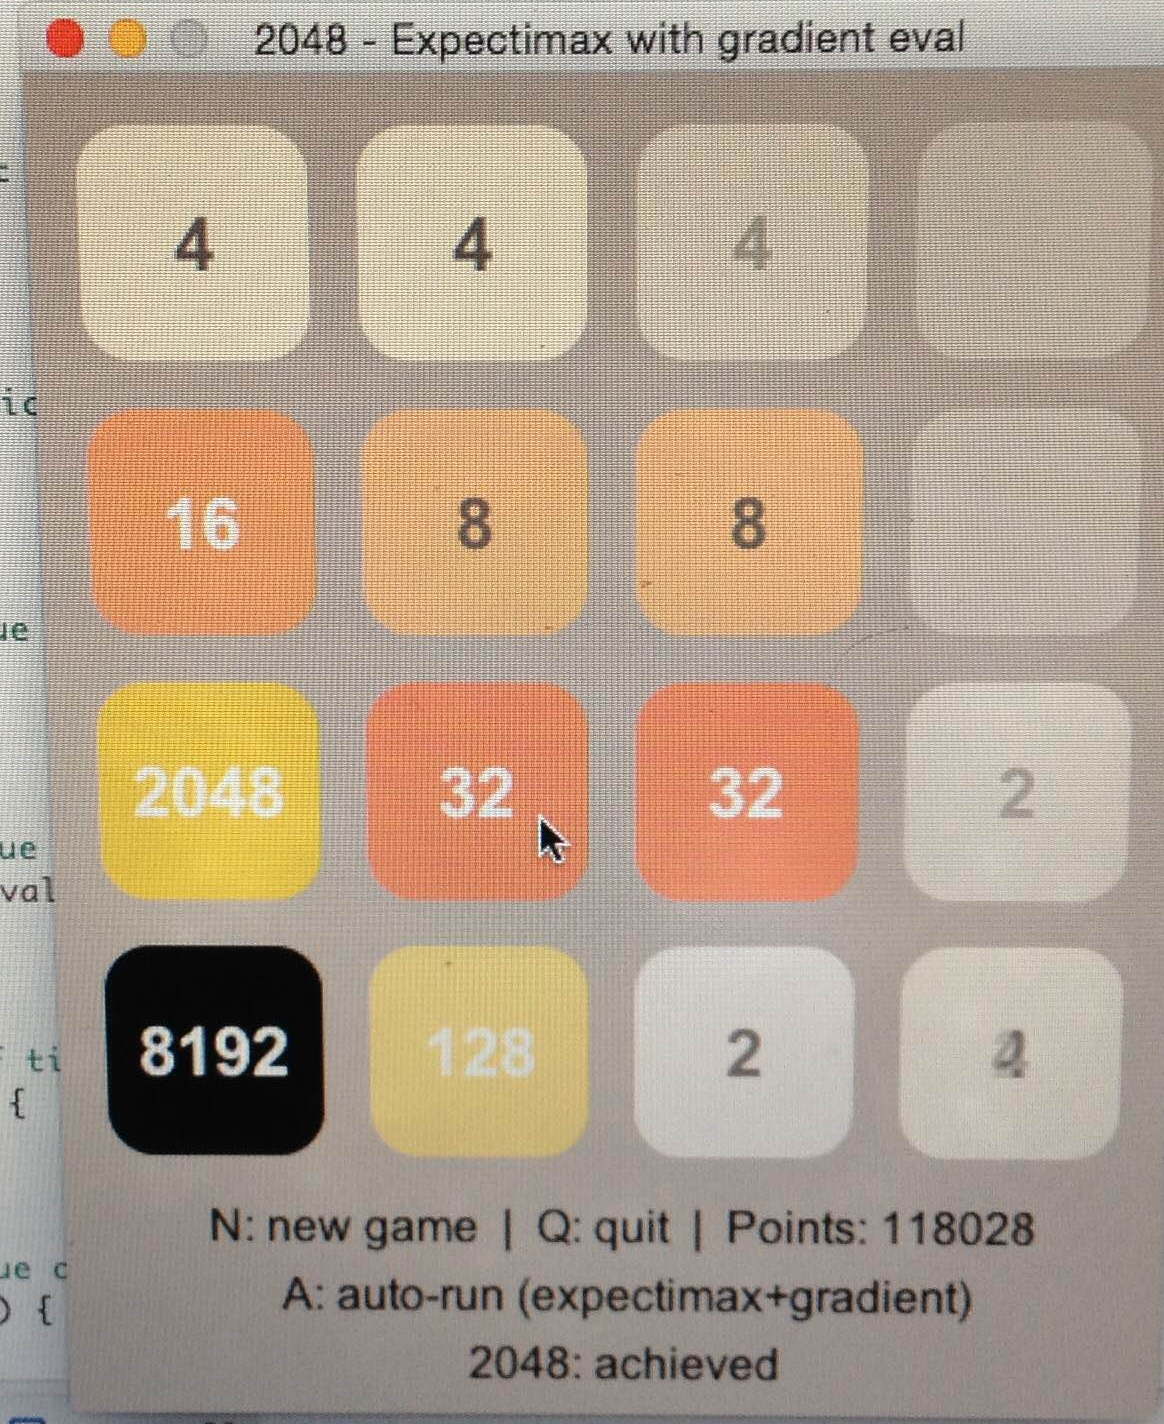
\includegraphics[keepaspectratio, height=6cm]{fig/8192.png}
\caption{Example solver and board}
\label{fig:max}
\end{figure}


\bibliographystyle{IEEEtran}
% \bibliography{IEEEabrv,../bib/paper}
\begin{thebibliography}{1}
\bibitem{brutesolver}
    ``ronzil'' \emph{2048-AI}, \textit{\url{https://github.com/ronzil/2048-AI}}.\hskip 1em plus
  0.5em minus 0.4em\relax GitHub
\end{thebibliography}

\end{document}
